\documentclass[11pt]{report}
\usepackage{textcomp}

\usepackage{titlesec}
\titlespacing*{\section}
{0pt}{\baselineskip}{0em}
\titlespacing*{\subsection}
{0pt}{\baselineskip}{0em}

\usepackage{geometry}
\geometry{left=1in, right=1in, top=1in, textheight=9in}

\usepackage{enumitem}
\newlist{steps}{enumerate}{1}
\setlist[steps, 1]{wide=0pt, leftmargin=\parindent, label=Step \arabic*:}

\usepackage{fancyhdr}
\fancypagestyle{plain}{%
    \fancyhf{} % clear all header and footer fields
    \fancyfoot[C]{\sffamily\fontsize{.75em}{.75em}\selectfont\thepage} % except the center
    \renewcommand{\headrulewidth}{0pt}
    \renewcommand{\footrulewidth}{0pt}
}
\pagestyle{plain}

\usepackage{graphicx}
\graphicspath{ {./media/} }

\usepackage{setspace}
\doublespacing

\usepackage{minted}
\usepackage{xcolor}
\definecolor{LightGray}{gray}{0.9}

% make fancy title page
\makeatletter
\newcommand{\@labsection}{000}
\newcommand{\labsection}[1]{
    \renewcommand{\@labsection}{#1}
}

\newcommand{\@labnumber}{0}
\newcommand{\labnumber}[1]{
    \renewcommand{\@labnumber}{#1}
}

\newcommand{\@shortsubmitted}{1/1/70}
\newcommand{\shortsubmitted}[1]{
    \renewcommand{\@shortsubmitted}{#1}
}

\lfoot{\footnotesize \textit{University of Arkansas \\ EECS Department}}
\rfoot{\footnotesize \textsl{\@shortsubmitted}}

\renewcommand{\maketitle}{
    \newgeometry{left=1in, right=1in, top=1.75in, textheight=8.25in}
    \singlespacing
    \begin{center}
        {\huge \bf CSCE 22104} \\
        \vspace{2.5em}
        {\Large \bf Lab Report} \\
        \vspace{2em}
        \noindent\rule{20em}{0.4pt} \\
        \vspace{1em}
        {\Large \@author} \\
        \vspace{.75em}
        {\normalsize ID: 011019116} \\
        \vspace{.75em}
        {\normalsize Lab Section \@labsection} \\
        \vspace{.75em}
        {\normalsize Lab \@labnumber} \\
    \end{center}
    \newpage
    \restoregeometry
}

\makeatother


% TEXTWIDTH = 100
\begin{document}
\title{Lab Report 8}
\author{Brent Marcus Orlina}

\labsection{001}
\labnumber{8}

\shortsubmitted{4/9/25}

\maketitle

\section*{Introduction}
This lab's goal was to implement a control block and sign extension components to support two
additional instructions \verb|addi| and \verb|subi|, with opcodes \verb|0100| and \verb|0101|
respectively. These two new instructions uses the last four bits of the instruction as an immediate
value instead of an address for a register.

The control block component should take in the first four bits of the instruction, representing the
opcode of the instruction and output the two-bit opcode used in the ALU, and which source should be
used in the second operand of the ALU, the data in register RT or the immediate value. The sign
extension component should take in the last four bits of the instruction, representing as the
immediate value, and extend it to 16 bits, taking into account its sign. The two components should
then be able to be combined with the CPU previously created from Lab 7.

\section*{Approach}
\begin{listing}[h!]
    \inputminted[
        frame=lines,
        breaklines,
        linenos,
        tabsize=4,
        fontsize=\footnotesize,
        bgcolor=LightGray
    ]{vhdl}{./media/control.vhd}
    \caption{The control block component's implementation.}
    \label{listing:control}
\end{listing}

Listing \ref{listing:control} shows the control block component's implementation. It takes in the
four-bit opcode through the input port \verb|op| and outputs the ALU opcode and ALU source through
the output ports \verb|ctrl_alu_op| and \verb|ctrl_alu_src| respectively.

In the architecture, the ALU opcode is simply the last two bits of the instruction opcode and the
ALU source is the third bit of the instruction opcode. This works because the opcode for the
immediate and non-immediate instructions of addition and subtraction only differ in the third bit.
As a reminder, the opcodes for \verb|add| and \verb|sub| are \verb|0000| and \verb|0001| and the
opcodes for \verb|addi| and \verb|subi| are \verb|0100| and \verb|0101|. This allows the control
block to use the third bit to determine whether the content in register \verb|RT| or the immediate
value should be used as the source of data for the ALU. The ALU opcode remains the same whether the
content of register \verb|RT| or the immediate value.

\begin{listing}[h!]
    \inputminted[
        frame=lines,
        breaklines,
        linenos,
        tabsize=4,
        fontsize=\footnotesize,
        bgcolor=LightGray
    ]{vhdl}{./media/immext.vhd}
    \caption{The sign extension component's implementation.}
    \label{listing:immext}
\end{listing}

Listing \ref{listing:immext} shows the sign extension component's implementation. It takes in the
four-bit immediate value through the input port \verb|imm| and outputs the sign-extended through the
output port \verb|ext|.

In the architecture, it uses a 12-bit signal, \verb|extension|, as a placeholder for what value
should be concatenated to \verb|imm| to extend it to 16 bits. For positive numbers, zeroes can
simply be concatenated as the most significant bit to extend the number. For example the 4-bit
positive number in two's complement, \verb|0011|, can be extended to 16 bits by simply concatenating
twelve zeroes to the most significant bit resulting in \verb|0000 0000 0000 0011| which keeps the
value.

For negative numbers, a series of ones can be concatenated to the most significant bit to extend the
number. For example, the 4-bit negative number in two's complement, \verb|1001|, $-7$ in decimal
form, can be extended to 16 bits by simply concatenating twelve ones to the most significant bit,
resulting in \verb|1111 1111 1111 1001| which is still $-7$ in decimal form. In two's complement, if
the most significant bit is a \verb|1| then the number is a negative. This allows the sign-extension
component to simply check whether the most significant bit is a \verb|1| or a \verb|0| to see if it
must concatenate twelve ones or twelve zeros, as seen on line 11 of listing \ref{listing:immext}. On
line 12, \verb|ext| is set as the concatenation of the determined extension and the input immediate
value, done through the \verb|&| operator in VHDL.

\newpage

\begin{listing}[h!]
    \inputminted[
        frame=lines,
        breaklines,
        linenos,
        tabsize=4,
        fontsize=\footnotesize,
        bgcolor=LightGray
    ]{vhdl}{./media/CPU-signals.vhd}
    \caption{The signals used in the CPU implementation.}
    \label{listing:CPU-signals}
\end{listing}

Listing \ref{listing:CPU-signals} shows the new signals used for the CPU implementation.
The \verb|ALUOP| signal is used to determine the operation that the ALU executes, addition,
subtraction, and-operation, or the or-operation. The signal \verb|ALUSource| is the control signal
that determines which data should go into the second operand of the ALU. It is decided between the
data from the \verb|RT| register, in the \verb|RTData| signal, or the sign-extended immediate value
in the \verb|Immediate| signal. The ALUInput is the signal used to put the result of the decision
made by the \verb|ALUSource|, connecting to the second operand of the ALU. Finally, the
\verb|Immediate| signal holds the value of the sign-extended immediate value of the instruction.

\newpage

\begin{listing}[h!]
    \inputminted[
        frame=lines,
        breaklines,
        linenos,
        tabsize=4,
        fontsize=\footnotesize,
        bgcolor=LightGray
    ]{vhdl}{./media/CPU-decode.vhd}
    \caption{The instruction decode phase of the CPU implementation.}
    \label{listing:CPU-decode}
\end{listing}

Listing \ref{listing:CPU-decode} shows the instruction decode phase of the CPU implementation. This
connects the \verb|OP| signal to the control block, which outputs the results to the \verb|ALUOP|
and \verb|ALUSource| signals.

This phase also connects the signal \verb|RT| to the immediate extension component, outputting the
sign-extended immediate value. Normally, the signal \verb|RT|, which is the last four bits of the
instruction, represents the address of the \verb|RT| register. However, since the immediate value is
also in the last four bits of the instruction for the \verb|addi| and \verb|subi| instructions, it
also represents the immediate value in these instructions. Since the operands of the ALU are 16-bits
long, the input immediate value needs to be sign extended.

Finally, the signal \verb|ALUInput| is determined whether it uses the data in the \verb|Immediate|
signal or the \verb|RTData| signal. Since the immediate instructions \verb|addi| and \verb|subi|
both have a \verb|1| in the third bit of their opcodes, which is what the \verb|ctrl_alu_src| looks
at in the control block, the ALU should use the immediate value when \verb|ALUSource| is active and
\verb|RTData| when it is inactive.

\begin{listing}[h!]
    \inputminted[
        frame=lines,
        breaklines,
        linenos,
        tabsize=4,
        fontsize=\footnotesize,
        bgcolor=LightGray
    ]{vhdl}{./media/CPU-execute.vhd}
    \caption{The execution phase of the CPU implementation.}
    \label{listing:CPU-execute}
\end{listing}

Finally, \ref{listing:CPU-execute} shows the execution phase of the CPU implementation. The new
\verb|ALUInput| and \verb|ALUOP| signals are connected to the ALU's \verb|B| and \verb|S| ports. The
\verb|ALUInput| signal is connected to account for the use of the sign-extended immediate value for
the \verb|addi| and \verb|subi| instructions.

\section*{Experimentation}
The components were tested by writing a testbench for the CPU component. The testbench written
tested for given instructions for the CPU and were manually verified to be correct.

\newpage

\section*{Results \& Discussion}
\begin{figure}[h!]
    \centering
    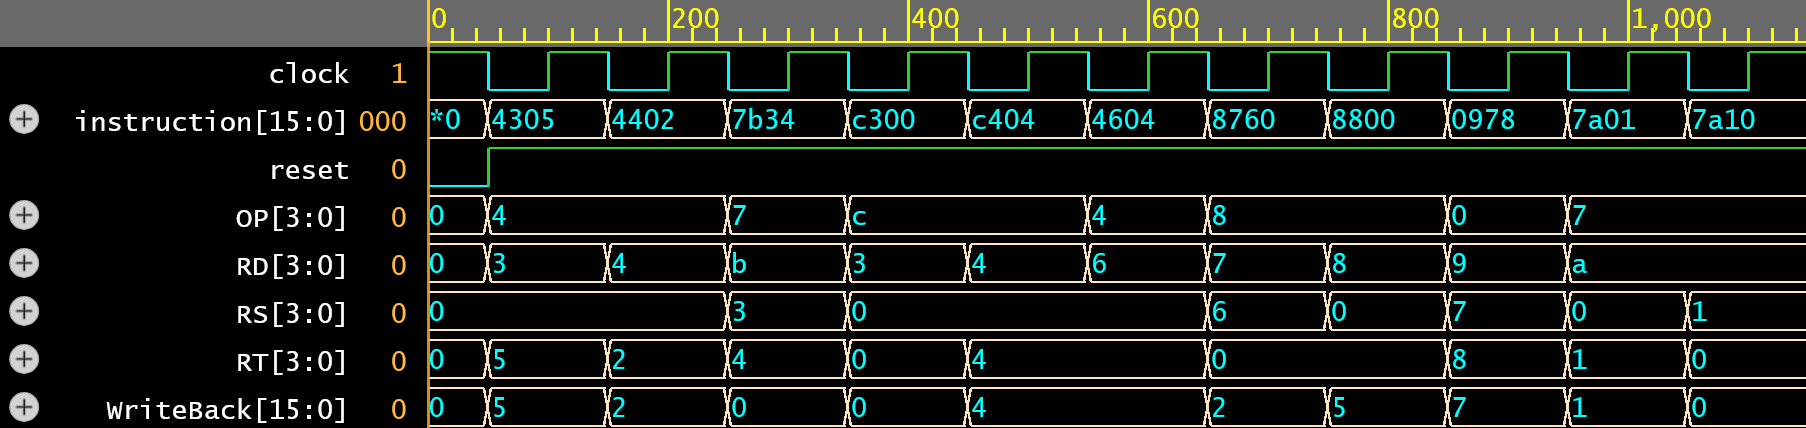
\includegraphics[width=0.95\textwidth]{CPU-waveform}
    \caption{The waveform for the CPU component.}
    \label{fig:CPU-waveform}
\end{figure}

\begin{table}[ht!]
    \centering
    \begin{tabular}{|l||c|c|c|c|c|} 
     \hline
     Instruction & op & rd & rs & rt & value (of rd) \\
     \hline
     \verb|ADD  R2, R1, R1| & \verb|0x0| & \verb|0x2| & \verb|0x1| & \verb|0x1| & \verb|2| \\ 
     \hline                                                                             
     \verb|ADDI R3, R2,  5| & \verb|0x4| & \verb|0x3| & \verb|0x2| & \verb|0x5| & \verb|7| \\
     \hline                                                                             
     %
     \verb|SUB  R4, R3, R2| & \verb|0x1| & \verb|0x4| & \verb|0x3| & \verb|0x2| & \verb|5| \\
     \hline                                                                             
     \verb|SUBI R5, R4, -4| & \verb|0x5| & \verb|0x5| & \verb|0x4| & \verb|0xC| & \verb|9| \\ 
     \hline                                                                             
     %
     \verb|AND  R6, R3, R5| & \verb|0x2| & \verb|0x6| & \verb|0x3| & \verb|0x5| & \verb|1| \\
     \hline                                                                             
     \verb|OR   R7, R5, R4| & \verb|0x3| & \verb|0x7| & \verb|0x5| & \verb|0x4| & \verb|13| \\
     \hline
     %             
    \end{tabular}
    \caption{Results of the CPU component testbench in table form.}
    \label{table:CPU-waveform_table}
\end{table}

The CPU component works as expected. Figure \ref{fig:CPU-waveform} shows the waveform of the CPU
component, correctly outputting the results of each operation. The waveform is in hex radix to
easily show the instruction in the current clock cycle and teh fact that the ALU does not have any
negative results. Table \ref{table:CPU-waveform_table} shows the waveform results in table form.

\section*{Conclusions}
Both the control block and signed-extension components worked correctly shown through the testbench
for the CPU. The knowledge learned from this lab was learning how to construct a control block
component and a signed-extension component to support two instructions, \verb|addi| and \verb|subi|
that uses an immediate value. The CPU was also rewired to support the use of these components and
the two new instructions.

% \newpage
% 
% \section*{References}
% \noindent
% [1]    Computer Organization 22104, EECS, University of Arkansas, “Lab 1,”  Sep. 17, 2024.
% 
% \noindent
% [2]    Computer Organization 22104, EECS, University of Arkansas, “Lab 2,”  Sep. 24, 2024.
% 
% \newpage
% 
% \section*{Appendix}
% \begin{figure}[h!]
%     \centering
%     \includegraphics[width=0.9\textwidth]{foo}
%     \caption{
%         Lorem ipsum dolor sit amet, qui minim labore adipisicing minim sint cillum sint consectetur
%         cupidatat.
%     }
%     \label{fig:foo}
% \end{figure}
% 
% \newpage
% 
% \begin{figure}[h!]
%     \centering
%     \includegraphics[height=0.4\textheight]{bar}
%     \caption{Lorem ipsum something something shorter sentence}
%     \label{fig:bar}
% \end{figure}
\end{document}
